\section{Experimental Results}
\label{sec:expResults}
%Results should be clearly displayed and should provide a suitable representation of your results for the points you wish to make. Graphs should be labeled in a legible font and if more than one result is displayed on the same graph then these should be clearly marked.   Please choose carefully rather than presenting every results. Too much information is hard to read and often hides the key information you wish to present. Make use of statistical methods when presenting results, where possible to strengthen the results.  Further, the format of the presentation of results should be chosen based on what issues in the results you wish to highlight. You may wish to present a subset in the experimental section and provide additional results in the appendix.

\subsection{Parameter Settings}
\label{subsec:parameterSettings_results}

Table \vref{table:parameterSettings2} shows the parameters tested, their candidate values and the selected value. The complete experimental steps with the corresponding results can be found in, Appendix \ref{appendixC}, Table \vref{table:pm1} and Table \vref{table:pm2}. 

    \begin{table}[H]
    \centering
    \begin{tabular}{|c|c||c|}
    \hline
    Parameters & Candidate values & Selected value\\
    \hline
    $s$ & 10, 50, 100, 125 & 50$^*$ \\
    $i$ & 10, 50 , 100, 125 & 125\\
    $E$ & 10\%, 25\% 50\%, 90\% & 25\% \\
    $CA$ & 0\%, 5\%, 10\%, 25\%, 50\%, 100\% & 25\% \\
    $AF$ & 0\%, 5\%, 10\%, 25\%, 50\%, 100\% & 5\% \\
    $p_{b}$ & 0.0, 0.1, 0.5, 0.9, 1.3 & 0.9 \\
    \hline
    \end{tabular}
    \caption {Results from the Parameter Settings Experiment}
    \begin{itemize}[noitemsep]
    \item[$^*$:]  Selected value is based on results presented in Figure \vref{fig:svsitesting} and Figure \vref{fig:svsiruntime} 
    \end{itemize}
    \label{table:parameterSettings2}
    \end{table}
    
\textbf{Evaluation of parameters}
\newline

As one can observe in Appendix \ref{appendixC}, Table \vref{table:pm1} and Table \vref{table:pm2}, the computed Confidence Interval does not become remarkably better after running the algorithm 50 times compared to 30. This makes it reasonable to conclude that the results regarding the parameters that were ran 30 times are valid.
\newline
%Because our confidence coefficient is sat to correspond to 95\%, we are able to say that we are 95\% confident that the true population parameter is between the lower and upper calculated values.

As one can observe in Table \vref{table:pm1}, increasing parameters $s$ and $i$ both increase the $TOTFIT$ value. The selected value for both parameters is 125 based on the best average produced $TOTFIT$. One aspect not considered in the initial parameter setting experiment is that the size of $s$ and $i$ affects each other. A colony of 50 ants with 100 iterations would produce close to similar results to 100 ants with 50 iterations. \emph{\color{blue}TODO: why does these affect eachother?}. The most optimal would be to observe the results when increasing the value of both these parameters. However, an increase in the swarm size or number of iterations both clearly affect the computational cost of the proposed algorithm. The average runtime of each run, with each candidate value, is presented in Figure \vref{fig:svsiruntime}. As one can see, there is a difference in the running time with a colony size of 125 versus 125 iterations. Between 100 and 125 ants the running time increases with 393 seconds, while between 100 and 125 iterations the running time increases with about 140 seconds. \emph{\color{blue}TODO: why is that?} Because the algorithm is going to be run an excessive amount of times when testing performance, and increasing both of these parameter values will result in an enormous runtime. As seen in \vref{table:pm1}, increasing the number of iterations increase the $TOTFIT$ value more than increasing the $S$ value. Due to this, the selected value of parameter $s$ is sat to \textit{50} and $i$ is sat to \textit{125}.

It is worth mentioning that values below 50 of parameter $s$, sometimes produce ant colonies were no ants satisfies the initial Constraint \ref{itm:criteriaConnectedGraph} described in Section \vref{sec:algoConstraints}. When $s$ is 10, this occurs on average 14.5\% of the iterations. If no ant satisfy the initial constraint, no ant is either evaluated, and their results will be invalid. 

\begin{figure}[H]
\begin{center}
  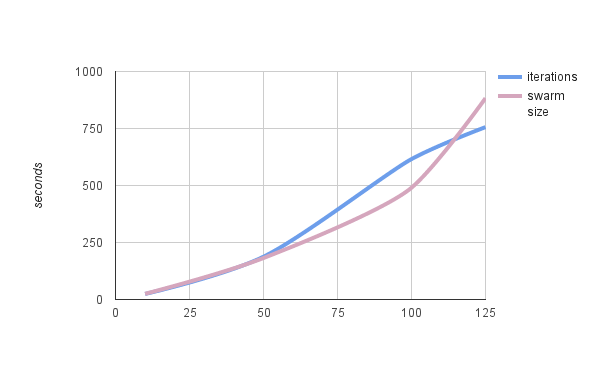
\includegraphics[width=5in]{assets/iterations_swarmsize_runtime.png}
  \end{center}
  \caption{Comparing Runtime when increasing the Swarm Size and the Number of Iterations}
  \label{fig:svsiruntime} 
\end{figure}

Observing the produced results of parameter $E$ in Table \vref{table:pm1}, evaporating 25\% of the pheromone each iteration gave the best average total fitness. The worst results were achieved when $E$ is 10\%. Evaporating too little of the pheromone\emph{\color{blue}TODO:}. As one can observe, the best produced results is achieved by a candidate value of 25\% to 50\%. The algorithm seems to benefit from the fact that a great amount of pheromone evaporates each iteration. We believe this is because it compensates for some of the randomness the parameter $CA$ produces, by quickly removing pheromone from edges that were once used, but later discarded. Even though the algorithm benefits from a large percentage of evaporated pheromones, it reaches a threshold were the percentage becomes too big. By removing 90\% of the pheromone an edge that is usually used a lot, but for some reason not used as much the given iteration, it is ``punished'' too hard. 
\newline

The value of $CA$ is sat to 25\% based on the results shown in Table \vref{table:pm2}, meaning there is a 25\% probability that an ant is declared ``crazy'' and thus makes completely random decisions. The results in Table \vref{table:pm2} shows that the algorithm benefits from the fact that some ants are declared crazy. However, if the probability is greater than 25\%, the average $TOTFIT$ results worsen. Not surprisingly, is this because half or more of the colony acts completely random, and the algorithm looses some of the performing boosting features from ACO, such as favoring edges frequently walked by other ants. \emph{\color{blue} TODO: gjøre en større deal ut av dette parameteret!!}
\newline

The amount of $AF$ determines the amount of Following Ants ($FA$) in the next iteration, and the $FA$ follow the same path as the best ants' paths unconditionally. Observing the results obtained in Table \vref{table:pm2}, the $TOTFIT$ value deteriorates when the amount of $AF$ becomes greater than 25\%. When the amount of $FA$ becomes too great, a relatively large number of normal ants will not be able to explore new (possibly better) routes in the next iterations, and the algorithm may suffer from a local optima. But as one also can see,  increasing the value computes better results than 0\%. Rewarding some good route sets seems to boost the algorithms performance, and 5\% is selected as the final parameter for $AF$. 

The value of $p_b$ is strongly dependent on the value of $AF$, because the more following ants, the more pheromone added to each edge in the best route sets. To ensure that rewarding edges with the selected amount of $AF$ ..., the value of $p_b$ was tested with the selected value of $AF$. As one can observe in Table \vref{table:pm2}, close to all $TOTFIT$ values increase when increasing the value of $p_b$. This makes it reasonable to conclude that awarding the best route sets' edges, is beneficial for the algorithm's performance.

